\documentclass[11pt,a4paper]{article}

\usepackage{../../templates/style}

\begin{document}

\begin{problem}{Trik}{standard input}{standard output}{1 second}{32 megabytes}

สมชายไปเที่ยวงานวัดแห่งหนึ่งซึ่งมีการแสดงมายากลในการสลับลูกบอลที่อยู่ในแก้วทึบ นักมายากลมีแก้วอยู่สามใบวางเรียงกัน โดยลูกบอลจะใส่ไว้ในแก้วใบซ้ายมือ นักมายากลจะสลับแก้วทีละสองใบด้วยความรวดเร็วแต่เราก็ยังสามารถมองได้ทันว่าเขาจับคู่ไหนหมุนอยู่บ้าง บังเอิญว่าสมชายเป็นโปรแกรมเมอร์จึงเขียนโปรแกรมเพื่อช่วยคำนวณตำแหน่งของลูกบอล โดยที่ได้ทำการเข้ารหัสการสลับของนักมายากลเป็นข้อมูล \textbf{A B C} ดังรูป

\begin{figure}[h]
\centering
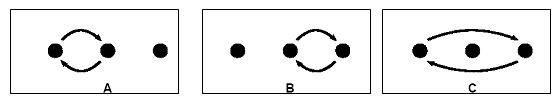
\includegraphics[width=1\textwidth]{../latex/img/0010/0010-1.png}
\end{figure}

\underline{\textbf{โจทย์}} จงเขียนโปรแกรมเพื่อรับรหัสการเคลื่อนย้ายแก้ว และหาตำแหน่งสุดท้ายของลูกบอล

\InputFile

\textbf{มีบรรทัดเดียว} จะมีสายอักขระความยาวไม่เกิน $50$ ตัวอักษรที่ประกอบด้วย \textbf{A B} หรือ \textbf{C}


\OutputFile

\textbf{มีบรรทัดเดียว} แสดง $1$ ถ้าลูกบอลอยู่แก้วซ้ายสุด, $2$ ถ้าลูกบอลอยู่แก้วใบกลาง และ $3$ ถ้าลูกบอลอยู่ในแก้วขวาสุด

\Examples

\begin{example}
\exmp{AB}{3}%
\exmp{CBABCACCC}{1}%
\end{example}

\newpage
\Source

Croatian Open Competition in Informatics

Contest 5 – February 17, 2007

\end{problem}

\end{document}